
\section{Oriented Point Reasoning Algebra With Granularity $m$ (\opra)}\label{sec:opra}

\kasten{
\subsubsection*{Oriented Point Relation Algebra (\opra) overview}
\begin{calcfeatures}
\feature{calculus identifier}{opra-}
\feature{calculus parameters}{granularity - number of partitioning lines (= number of planar relations / 2), must be $> 0$}
\feature{arity}{binary}
\feature{entity type}{oriented 2D points}
\feature{description}{relates two oriented points $a$ and $b$ with respect to granularity $m$}
\feature{base relations}{$[i,j]$ with $i, j$ $\in \{0,..,4m-1\}$, if $a$ and $b$ have different positions; $[i]$ with $i \in \{0,..,4m-1\}$ if they have the same position}
\lastfeature{references}{\citet{Moratz_Dylla_Frommberger_05_adjustable_Granularity,moratz06_opra}}
%\item[remarks]
\end{calcfeatures}
}

The domain of the Oriented Point Relation Algebra (\OPRAm{}) \citep{Moratz_Dylla_Frommberger_05_adjustable_Granularity,moratz06_opra} is the set of oriented points (points in the plane with an
additional direction parameter). The calculus relates two  oriented points
with respect to their relative orientation towards each other.
An oriented point
$\vec{O}$ can be described by its Cartesian coordinates $x_O, y_O \in {\mathbb{R}}$ and a direction $\phi_{\vec{O}} \in [0,2\pi]$ with respect to an absolute
reference direction and thus $D={\mathbb{R}}^2 \times [0,2\pi]$.

The \OPRAm{} calculus is suited for dealing with objects that have an intrinsic front or move in a particular direction and can be abstracted as points.
The exact set of base relations distinguished in  \OPRAm{} depends on the
granularity parameter $m\in \mathbb{N}$. For each of the two related oriented points, $m$ lines are used to partition the plane into $2m$ planar and $2m$ linear regions. Fig.~\ref{fig:OPRA} shows the partitions for the cases $m=2$
%(Fig.~\ref{fig:OPRA2})
(a) and $m=4$
%(\ref{fig:OPRA4})
(b). The orientation of the two points is depicted by the arrows starting at $\vec{A}$ and $\vec{B}$, respectively. The regions are numbered from 0 to $4m-1$; region 0 always coincides with the orientation of the point. An \OPRAm{} base relation $rel_{\mathcal{OPRA}_m}$ consists of a pair $(i,j)$ where
$i$ is the number of the region of $\vec{A}$ which contains $\vec{B}$, while $j$ is the number of the region of $\vec{B}$ that contains $\vec{A}$. These relations are usually written as $\vec{A} \; {\scriptscriptstyle m}\angle_{i}^{j} \; \vec{B}$ with $i,j\in \mathcal{Z}_{4m}$\footnote{$\mathcal{Z}_{4m}$ defines a cyclic group with $4m$ elements.}. Thus, the examples in Fig.~\ref{fig:OPRA} depict the relations $\vec{A} \; {\scriptscriptstyle 2}\angle_{7}^{1} \; \vec{B}$ and $\vec{A} \; {\scriptscriptstyle 4}\angle_{13}^{3} \; \vec{B}$. Additional base relations called \emph{same relations} describe situations in which the positions of both oriented points coincide. In these cases, the relation is determined by the number $s$ of the region of $\vec{A}$
into which the orientation arrow of $\vec{B}$ falls (as illustrated in Fig.~\ref{fig:OPRA2same}). These relations are written as $\vec{A} \; {\scriptscriptstyle 2}\angle s \; \vec{B}$ ($\vec{A} \; {\scriptscriptstyle 2}\angle 1 \; \vec{B}$ in the example).

The complete set $\mathcal{R}$ of \OPRAm{} relations is the power set
of the base relations described above.
% \marginpar{FD: $2^{[(4m)^2+4m]}$ sagen?}

\begin{figure}[tb!]
% \begin{center}
\begin{flushleft}
	\subfigure[$m=2$: $\vec{A} \; {\scriptscriptstyle 2}\angle_{7}^{1} \; \vec{B}$]{
% 	\subfigure[with $m=2$: $\vec{A} \; {\scriptscriptstyle 2}\angle_{7}^{1} \; \vec{B}$]{
		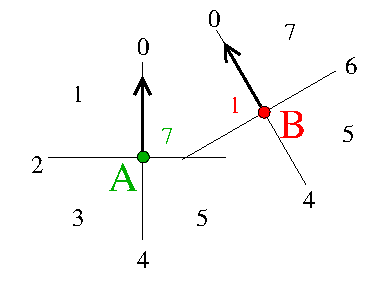
\includegraphics[width=0.307\textwidth]{OPRA2_Example}
		\label{fig:OPRA2}
	}
	\subfigure[$m=4$: $\vec{A} \; {\scriptscriptstyle 4}\angle_{13}^{3} \; \vec{B}$]{
% 	\subfigure[with $m=4$: $\vec{A} \; {\scriptscriptstyle 4}\angle_{13}^{3} \; \vec{B}$]{
		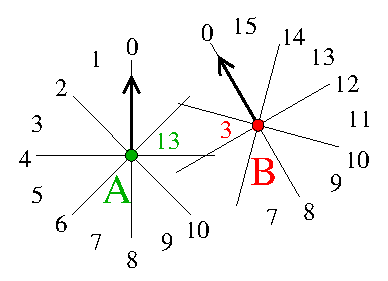
\includegraphics[width=0.307\textwidth]{OPRA4_Example}
		\label{fig:OPRA4}
	}
	\subfigure[case where $\vec{A}$ and $\vec{B}$ coincide: $\vec{A} \; {\scriptscriptstyle 2}\angle 1 \; \vec{B}$]{
		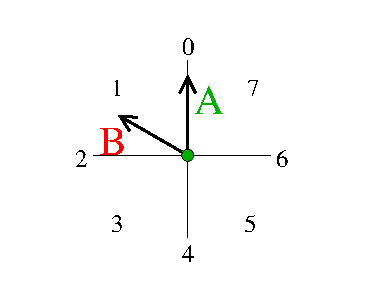
\includegraphics[width=0.307\textwidth]{OPRA2_ExampleSame}
		\label{fig:OPRA2same}
	}
	\caption{Two oriented points related at different granularities.}
	\label{fig:OPRA}
\end{flushleft}
% \end{center}
\end{figure}
